\documentclass{standalone}
\usepackage{mathpazo}
\usepackage[american voltages]{circuitikz}

\begin{document}
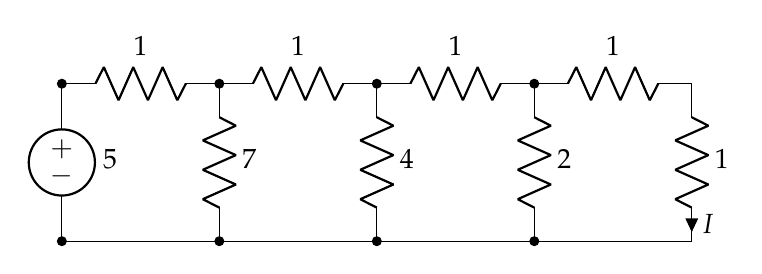
\begin{tikzpicture}
  \draw
  (0,0) to [R, *-*, l=1] ++(2,0)
  to [R, -*, l=1] ++(2,0)
  to [R, -*, l=1] ++(2,0)
  to [R, -, l=1] ++(2,0)
  to [R, -, l=1, i= $I$] ++(0, -2)
  to [short, -*] ++(-2,0)
  to [short, -*] ++(-2,0)
  to [short, -*] ++(-2,0)
  to [short, -*] ++(-2,0);
  \draw
  (2,0) to [R, l=7] ++(0, -2)
  (4,0) to [R, l=4] ++(0, -2)
  (6,0) to [R, l=2] ++(0, -2);
  \draw
  (0,0) to [V, l=5] (0,-2);
  \end{tikzpicture}
\end{document}